\section{Background} \label{sec_background}
\subsection{Decomposition Schemes}
Large multipliers are typically built by decomposing the computation into smaller multipliers that match the target architecture, trading multiplier count against shift-and-add overhead.
\subsubsection{Schoolbook Decomposition}
Schoolbook decomposition forms a $2n\times 2n$ product using four $n\times n$ partial products (Equation~\ref{schoolbook_eq}). Let $A=(A_1\ll n)+A_0$ and $B=(B_1\ll n)+B_0$ (Figure~\ref{fig:karatsuba_vs_schoolbook}).
\begin{equation} \label{schoolbook_eq}
\begin{split}
    \mathit{Schoolbook}(A \times B) = & P1 +(P2 << 2n) \\
                &+ ((P3+ P4) << n) \\
\end{split}
\end{equation}
This approach scales quadratically (e.g., nine multipliers for a $3\times 3$ split) and relies on shift-and-add logic to combine partial products.
Equation~\ref{schoolbook_eq} can be rearranged to save an addition by using concatenation~\cite{zhangIMpressLargeInteger2022} to obtain Equation~\ref{trick_schoolbook_eq}.


\begin{equation} \label{trick_schoolbook_eq}
    (P1 +(P2 << 2n)) = \{P2, P1\}
\end{equation}

\subsubsection{Karatsuba Decomposition}
Karatsuba~\cite{karatsubaOriginalPaper} reduces the $2\times2$ case from four multipliers to three by replacing one multiplication with additions/subtractions.
One product is typically $(n{+}1)$ bits wide.
Figure~\ref{fig:karatsuba_vs_schoolbook} compares Schoolbook and Karatsuba for a $2n \times 2n$ multiplier. 
Karatsuba extends to larger grids (e.g., $3\times3$), saving three multipliers relative to Schoolbook (uses $9$ multipliers).
\begin{equation} \label{karatsuba_eq}
\begin{split}
    \mathit{Karatsuba}(A_0  B_1 + A_1  B_0) = P3-P1-P2
\end{split}
\end{equation}


\begin{figure}[t]
    \centering
    \begin{subfigure}{0.48\columnwidth}
        \centering
        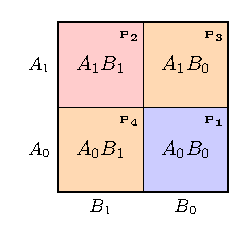
\includegraphics[width=\textwidth]{figures/decomposition/schoolbook_decomposition_standalone.pdf}
        \caption{Schoolbook decomposition.}
        \label{fig:schoolbook_decomp}
    \end{subfigure}%
    \hfill
    \begin{subfigure}{0.48\columnwidth}
        \centering
        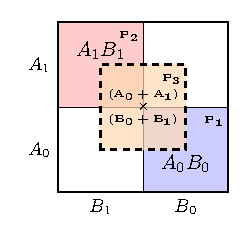
\includegraphics[width=\textwidth]{figures/decomposition/karatsuba_decomposition_standalone.pdf}
        \caption{Karatsuba decomposition.}
        \label{fig:karatsuba_decomp}
    \end{subfigure}
\caption{Comparison of Schoolbook and Karatsuba decomposition schemes for a $2n \times 2n$ multiplier.}
\label{fig:karatsuba_vs_schoolbook}
\end{figure}

%%%%%%%%%%%%%%%%%%%%%%%%%%%%%%%



The $(n{+}1)$-bit multiply can be implemented using an $n$-bit multiplier plus lightweight logic by splitting each operand into an $n$-bit part and a 1-bit part (Figure~\ref{fig:karatsuba_nplus1_decomposition}). The $n\times1$ and $1\times1$ terms reduce to AND gates, and non-overlapping terms can be concatenated (Equation~\ref{trick_schoolbook_eq}). Placing the $n\times n$ multiplier on the LSB side (Figure~\ref{fig:karatsuba_lsb}) reduces the widest adder from $2n{+}1$ to $n{+}1$ bits.



\begin{figure}[t]
    \centering
    \begin{subfigure}{0.45\textwidth}
        \centering
        
\includegraphics[width=\textwidth]{figures/decomposition/nplus1bitMultNMSB_standalone.pdf}
        \caption{The $n\times n$ multiplier is used for the MSB (The adder tree needs a $2n+1$-bit adder).}
        \label{fig:karatsuba_msb}
    \end{subfigure}
    \hfill
    \begin{subfigure}{0.45\textwidth}
        \centering
        
\includegraphics[width=\textwidth]{figures/decomposition/nplus1bitMultNLSB_standalone.pdf}
        \caption{The $n\times n$ multiplier is used for the LSB (The adder tree needs a $n+1$-bit adder).}
        \label{fig:karatsuba_lsb}
    \end{subfigure}
    \caption{$n+1$-bit multiplier used in Karatsuba decomposition. The grey areas denote the shift amount for each partial product (added zeros). The dotted red rectangle denotes concatenation}
    \label{fig:karatsuba_nplus1_decomposition}
\end{figure}


%%%%%%%%%%%%%%%%%




\subsection{DSP Block Consideration}
\subsubsection{Overview and Applications}
A DSP block is a hard FPGA primitive optimized for high-frequency multiply and add/accumulate operations. Modern families increased multiplier widths (e.g., $25\times18$ in Virtex-5/6/7, $27\times18$ in UltraScale(+), and $27\times24$ in Versal).
They are widely used in FIR filters, ML inference, and scientific signal processing~\cite{xilinxVirtex-4DSPExplainedFPGA,ghiasiDSPEfficientCNNFPGA2020}; some families also support floating-point modes~\cite{pascaFloatingPointDSPBlock2015}.


\subsubsection{AMD DSP Slice Architecture}
An AMD DSP slice integrates a pre-adder (not shown nor used in this work), multiplier, multiplexers, and an ALU (Figure~\ref{fig:cascade_comparison}).
Control signals (e.g., OPMODE/ALUMODE) select the datapath/ALU expression~\cite{UltraScaleArchitectureDSP2021}, and optional pipeline registers trade latency for throughput (enabling all four registers yields maximum throughput).
Cascaded ports (e.g., PCIN/PCOUT) support efficient column-wise chaining.
Correct multiplier and cascade behavior requires routing the multiplier partial products through the $X$ and $Y$ multiplexers while selecting the appropriate $Z$ source (e.g., PCIN) via OPMODE.


% \begin{equation} \label{final_alu_output_eq}
% \begin{split}
%     \mathit{ALU\ Expression}=\begin{cases}
%     Z +W+X+Y +C_{in}\\ 
%                         Z -(W+X+Y +C_{in})\\ 
%                         -Z +(W+X+Y +C_{in})\\ 
%                         \text{not}(Z +W+X+Y +C_{in})            
%     \end{cases}
% \end{split}
% \end{equation}


% \begin{equation} \label{final_dsp_output_eq}
% \begin{split}
%     \mathit{DSPOut} =\begin{cases}
%     C \pm (B\times(D\pm A)\ +\ W + C_{in})\\ 
%     C \pm (A\times(D\pm B)\ +\ W + C_{in})\\
%     C \pm (B\times(D\pm B)\ +\ W + C_{in})\\
%     C \pm (A\times(D\pm A)\ +\ W + C_{in})\\
%     C \pm ((D\pm B)^2\ +\ W + C_{in})\\
%     C \pm ((D\pm A)^2\ +\ W + C_{in})
%     \end{cases}
% \end{split}
% \end{equation}



\subsubsection{Chaining DSP Slices} \label{sec_dsp_cascade}
More than one DSP slice can be chained to create wider multipliers.
For instance, two DSP slices can be chained to perform a $44\times18$ multiplication.
Assuming that we have two inputs $K$ of size $44$ bits and $M$ of size $18$ bits,
$K$ is split into two parts: the lower $17$ bits ($K_L$) and the upper $27$ bits ($K_H$).
To fit within the $48$-bit datapath and leverage the built-in 17-bit right shift, rewrite the accumulation as in Equation~\ref{dsp_cascade_shift_eq}.

\begin{equation} \label{dsp_cascade_shift_eq}
\begin{split}
    P1 &= (K_L\times M), \quad P2 = (K_H \times M)\\
    K\times M &=  \{(P2 + (P1 >>17)),
            \ P1[16:0]\}
\end{split}
\end{equation}

Figure~\ref{fig:cascade_comparison} contrasts two chaining options: PCOUT-to-PCIN cascading versus routing P-to-C.
With PCOUT-to-PCIN, S1 cascades PCOUT to S2 PCIN and S2 uses the built-in $17$-bit shift.
Signal synchronization requires delaying $K_H$, $M$, and the extracted LSBs from P1, resulting in a 5-cycle latency.
Because the cascade path supports only 0 or 17-bit shifts, other shifts use the P-to-C path which requires LUT-based shift/sign-extension (ExSRn) and route S1's P to S2's C, typically adding an extra pipeline stage.


\begin{figure}[t]
    \centering
    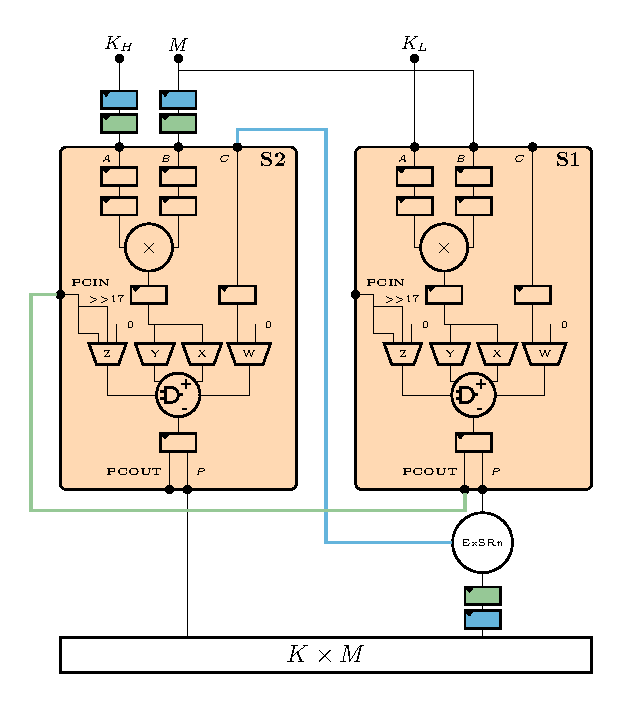
\includegraphics[width=0.9\columnwidth]{figures/dsp48e2/cascade_comparison_standalone.pdf}
    \caption{Comparison of cascade paths. The ExSRn block extracts the first n bits of P and passes it to the register, and also shifts P right by n bits and sign extends and passes it to C input. Blue connection and registers denote the P-to-C path while blue connection and added register denote the PCOUT-to-PCIN cascade path.}
    \label{fig:cascade_comparison}
\end{figure}
%%%%%%%%%%%%%%%%%%%%%%%%%%%%%%%%%%%%%%%%%%%%%%%%%%%%%%%%%%


\subsection{Signed vs Unsigned Multiplication} \label{sec_sign_unsigned_mult}
When constructing large multipliers from smaller bases, signedness must be handled carefully.
In decomposition, only the parts containing MSB should be treated as signed (for a signed multiplication); all other partial products must be computed as unsigned.
A signed $n$-bit multiplier can be used as an unsigned $(n{-}1)$-bit multiplier by zero-padding the MSB.
%%%%%%%%%%%%%%%%%%%%%%%%%%%%%%%%%%%%%%%%%%%%%%%%%%%


\subsection{IP Multipliers} \label{sec_ip_background}
AMD provides a Vivado IP multiplier~\cite{xilinxincIPMultiplier2015} that generates parameterized unsigned multipliers up to $64\times64$ bits, with options to optimize for frequency or resource utilization and a chosen pipeline depth.
For sizes larger than $47\times47$ bits, only the performance-optimal design is offered; it achieves maximum DSP frequency but consumes many DSP blocks.